% !TEX root = main.tex

\section{Evaluating the approaches}\label{sec:evaluation}

\subsection{Evaluation methods}

To evaluate and compare the approaches different techniques are used: 
\begin{itemize}
	\item \textbf{K-Fold Cross Validation}: where the data is randomly divided into folds and one of those is used for testing while the rest for training. It is often used in papers containing ML approaches to ranking alerts, though it has its drawbacks. As shown in \cite{performance_method_bug} and as can be seen on \cref{kfold_vs_release}, this approach uses dependent variables (most of the extracted features), that may not be available at prediction time in a real world scenario. That can lead to unreliable and excessively optimistic results. Cross Validation was only used for selecting the right classifier for this task, and not for evaluating the ranking approaches.
	\item \textbf{Release/Revision based testing}: avoids the drawback of the previous method, by using a \textit{"horizontal"} train/test strategy. We fix a certain point in time (revision or release) which defines what the train set (before that point) and test set (after that point) will be. This trains the algorithms with more realistic data, but it also has its drawbacks. In a scenario where the dataset is imbalanced, a \textit{"horizontal"} 80/20\% split may leave us with very little data. Also, unlike in cross validation, we cannot train and test different models.
	
	\begin{figure}[H]
		\centering
		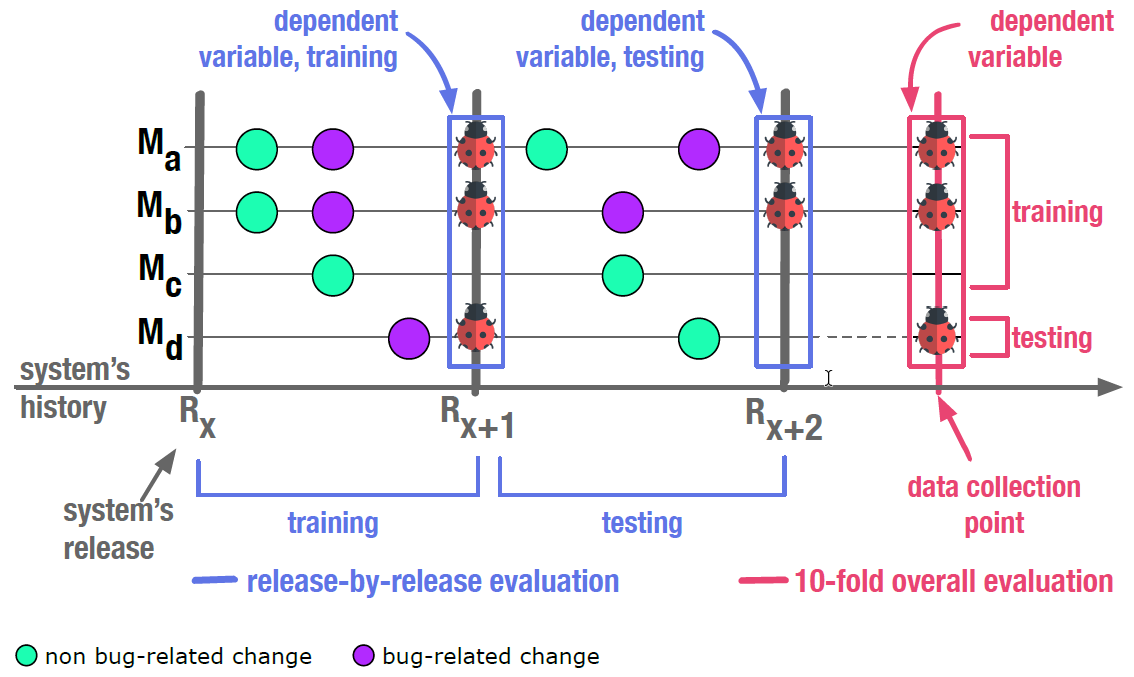
\includegraphics[scale=0.3]{./src/release_based_testing.png}
		\caption{Release-based vs K-Fold (\cite{performance_method_bug})}
		\label{kfold_vs_release}
	\end{figure}
	
	\item \textbf{Average FP to TP (\cite{correlation_exploitation})}: Let N be the total number of actionable alerts in a set of reports, and $FP_j$ is the cumulative
	number of false positives to find the \textit{j}th actionable alert.
	
	\begin{gather*}
	AVG_{FP-TP}(R) = \frac{\sum_{i=1}^{N} FP_j}{N}
	\end{gather*}
	
	\item \textbf{S(R) metric (\cite{z-ranking})}: Let \textit{N} be
	the total number of alerts and \textit{act} the number of actionable ones. Let \textit{R(i)} denote the cumulative number of actionable alerts found by a ranking scheme \textit{R} on the \textit{i}th inspection. \\
	\begin{gather*}
	S(R) = \sum_{i=1}^{N} [min(i,act) - R(i)]
	\end{gather*}
	\item \textbf{Random comparison}: where we compare if the ranking produced by a model is better than a random order of alerts. We calculate that by using the two previously defined metrics.
	\item \textbf{Fault detection rate curve}: the curve of a model is formed by plotting the number of actionable alerts found within the first N inspections.
	
	% \item Feedback-Rank paper has some approaches.
\end{itemize}

\subsection{Evaluation Metrics}

Along with the classic evaluation metrics like \textit{accuracy}, \textit{precision} and \textit{recall}, other metrics are used that are more appropriate for imbalanced data (\cite{comparison_metrics}, \cite{iba_metric}). 


\begin{gather*}
Sensitivity = \frac{TP}{TP + FN}\\
Specificity = \frac{TN}{FP + TN}\\
G-Mean = \sqrt{Sensitivity * Specificity}
\end{gather*} 
Sensitivity, or True Positive Rate is the percentage of positive examples which
are correctly classified.\\
Specificity, or True Negative Rate, is the percentage of negative examples which are correctly classified.\\
G-Mean is the geometric mean of the sensitivity and specificity.


\begin{gather*}
AUC = \frac{Sensitivity + Specificity}{2} \qquad (*approximation \ using \ trapezoid \ rule)
\end{gather*} 
The \textit{AUC} of a binary classifier is equivalent to the probability that the classifier will rank a randomly chosen positive instance higher than a randomly chosen negative instance.


\begin{gather*}
IBA_{\alpha} = (1 + \alpha * (Sensitivity - Specificity)) * Sensitivity * Specificity
\end{gather*} 
The \textit{Index of Balanced Accuracy} used for evaluating learning processes in two-class imbalanced domains. The
method combines an unbiased index of its overall accuracy and a measure about
how dominant is the class with the highest individual accuracy rate.


%\subsubsection{Preparing the dataset}
%\textbf{TODO: EVALUATE ENCODING METHODS}

\subsection{Results of individual tools}

Experiments were run by training methods on the first 80\% items of the dataset and testing on the remaining 20\%. In the first two methods a \textit{Random Forest} classifier was used. We chose it because of its good performance in terms and speed.

\subsubsection{Actionable Alerts}

Different balancing algorithms were applied to the training set and \textit{Random Forest} was used as a classifier, yielding the following results of the test set (*):

\begin{table}[H]
	\centering
	\begin{tabular}{@{}ccccccc@{}}
		\toprule
		& \textbf{Precision} & \textbf{Recall} & \textbf{Specificity} & \textbf{F1-Score} & \textbf{Geometric} & \textbf{IBA}  \\ \midrule
		\textit{Random Over Sampler}  & 88\%               & 87\%            & 75\%                 & 86\%              & 79\%               & 63\%          \\
		\textit{Random Under Sampler} & 91\%               & 90\%            & 82\%                 & 90\%              & 85\%               & 73\%          \\
		\textit{SMOTE}                & \textbf{94\%}      & \textbf{94\%}   & \textbf{90\%}        & \textbf{94\%}     & \textbf{92\%}      & \textbf{85\%} \\
		\textit{ADASYN}               & 90\%               & 90\%            & 81\%                 & 89\%              & 85\%               & 72\%          \\
		\textit{SMOTEENN}             & 89\%               & 88\%            & 77\%                 & 87\%              & 81\%               & 66\%          \\
		\textit{SMOTETomek}           & 89\%               & 88\%            & 77\%                 & 87\%              & 81\%               & 67\%          \\ \bottomrule
	\end{tabular}
\end{table}

\textit{(*) calculated using the balanced classification report of imblearn}


\begin{figure}[H]
	\begin{subfigure}{\textwidth}
		\centering
		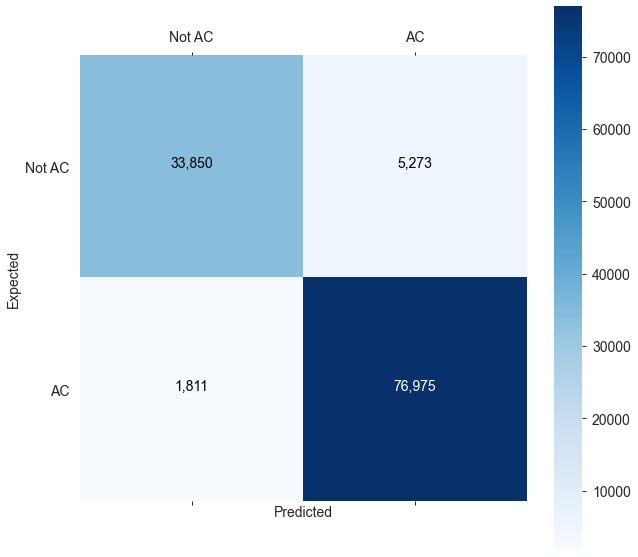
\includegraphics[scale=0.3]{./src/actAlerts/actalerts_smote_cm.png}
		\caption{Confusion matrix of test set for SMOTE balanced training set}\label{}
	\end{subfigure}\\
	\begin{subfigure}{.5\textwidth}
		\centering
		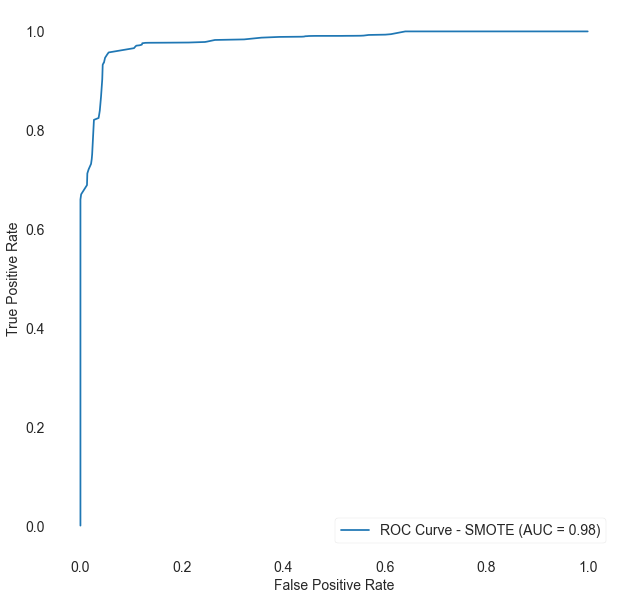
\includegraphics[scale=0.3]{./src/actAlerts/actalerts_smote_roc.png}
		\caption{ROC Curve for SMOTE balanced training set}\label{}
	\end{subfigure}%
	\begin{subfigure}{.5\textwidth}
		\centering
		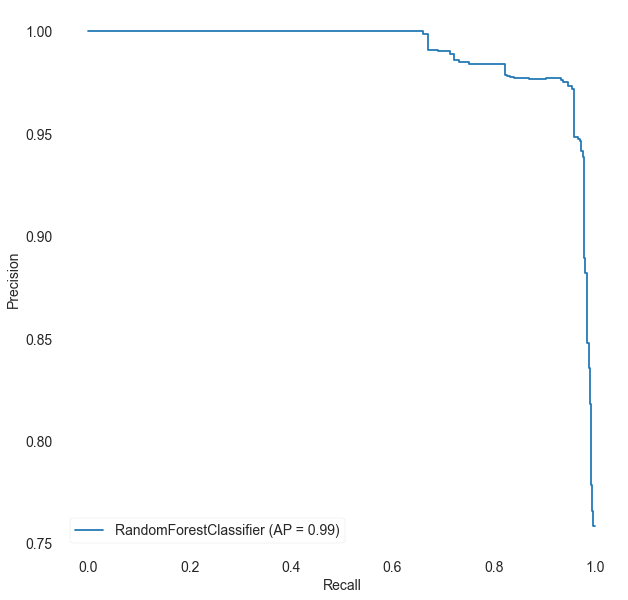
\includegraphics[scale=0.3]{./src/actAlerts/actalerts_smote_pr.png}
		\caption{Precision/Recall curve for SMOTE balanced training set}\label{}
	\end{subfigure}  
\end{figure}

Alerts are ranked based on the probabiliy score produced by the classifier for the prediction target (actionable or not).
In order to evaluate the ranking, two metrics are used to compare the ranked alerts with a random order. The experiments are run multiple times (by shuffling the random order and calculating the metrics again).\\

The order produced by the Random Forest classifer always outperforms the random order.
\begin{table}[H]
	\centering
	\begin{tabular}{@{}lll@{}}
		\toprule
		& \textbf{S(R) metric} & \textbf{Average FP to TP} \\ \midrule
		\textit{Better than random (Top 1000 alerts)} & 1000 out of 1000     & 1000 out of 1000          \\
		\textit{Better than random (All alerts)}      & 10 out of 10         & 10 out of 10              \\ \bottomrule
	\end{tabular}
\end{table}

Furthermore, the order of the ranked alerts if compared against the random and perfect order by using the cumulative graph.
\begin{figure}[H]
	\centering
	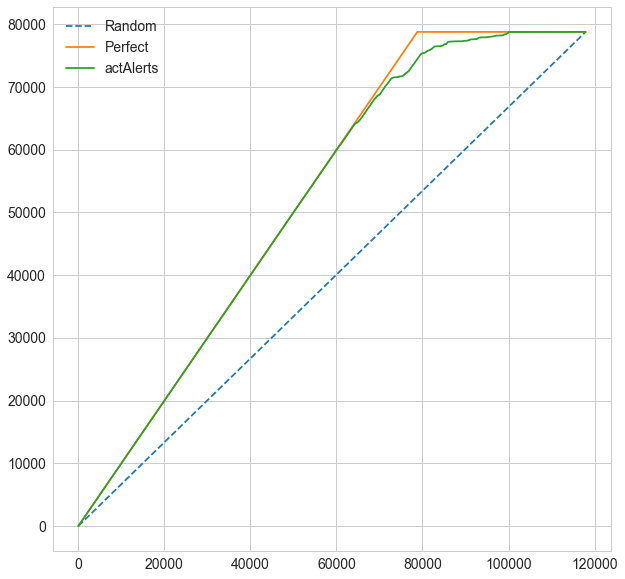
\includegraphics[scale=0.4]{./src/actAlerts/cumulative_graph_all.png}
	\caption{Cumulative graph for all sorted alerts}
	\label{}
\end{figure}


\subsection{Method Bug Prediction}

Different balancing algorithms were applied to the training set and \textit{Random Forest} was used as a classifier. The following results show the score of the classifier in predicting if a method will be buggy in the future:

\begin{table}[H]
	\centering
	\begin{tabular}{@{}ccccccc@{}}
		\toprule
		& \textbf{Precision} & \textbf{Recall} & \textbf{Specificity} & \textbf{F1-Score} & \textbf{Geometric} & \textbf{IBA}  \\ \midrule
		\textit{Random Over Sampler}  & \textbf{70\%}      & \textbf{70\%}   & \textbf{55\%}        & \textbf{70\%}     & \textbf{60\%}      & \textbf{37\%} \\
		\textit{Random Under Sampler} & 65\%               & 70\%            & 39\%                 & 66\%              & 42\%               & 18\%          \\
		\textit{SMOTE}                & 68\%               & 70\%            & 48\%                 & 69\%              & 53\%               & 29\%          \\
		\textit{ADASYN}               & 67\%               & 70\%            & 45\%                 & 68\%              & 51\%               & 26\%          \\
		\textit{SMOTEENN}             & 66\%               & 70\%            & 41\%                 & 67\%              & 45\%               & 21\%          \\
		\textit{SMOTETomek}           & 68\%               & 70\%            & 47\%                 & 69\%              & 52\%               & 28\%          \\ \bottomrule
	\end{tabular}
\end{table}

\begin{figure}[H]
	\begin{subfigure}{\textwidth}
		\centering
		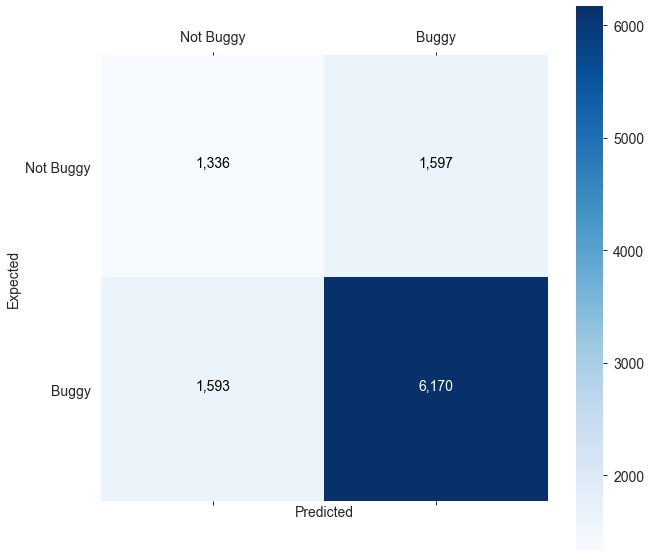
\includegraphics[scale=0.3]{./src/methodBug/methodbug_rover_cm.png}
		\caption{Confusion matrix of test set for Random Oversampling balanced training set}\label{}
	\end{subfigure}\\
	\begin{subfigure}{.5\textwidth}
		\centering
		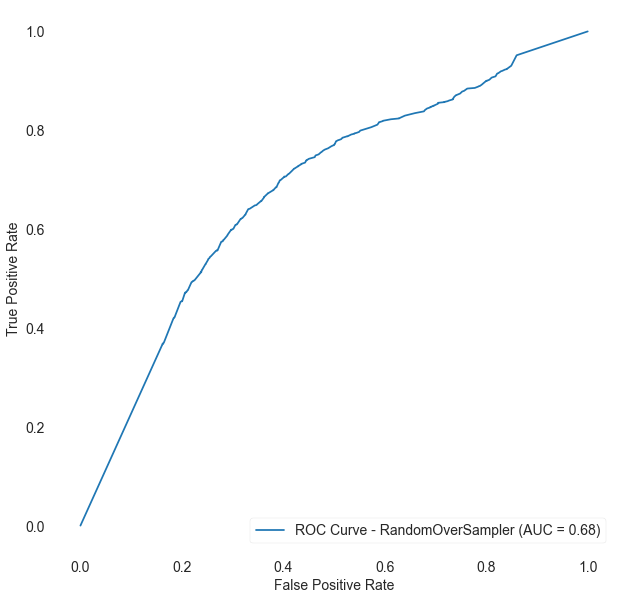
\includegraphics[scale=0.3]{./src/methodBug/methodbug_rover_roc.png}
		\caption{ROC Curve for Random Oversampling balanced training set}\label{}
	\end{subfigure}%
	\begin{subfigure}{.5\textwidth}
		\centering
		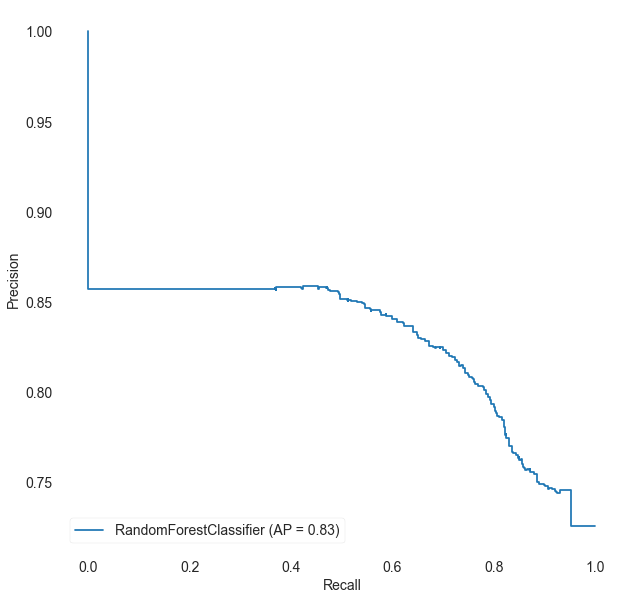
\includegraphics[scale=0.3]{./src/methodBug/methodbug_rover_pr.png}
		\caption{Precision/Recall curve for Random Oversampling balanced training set}\label{}
	\end{subfigure}  
\end{figure}


After calculating the probability of a method being buggy on the test set, we merge that set with the one containing actionable alerts. The goal is to see if ranking alerts higher when they belong to a bug prone method is useful in terms of predicting if that alert will be actionable in the future.

Alerts are ranked based on the probabiliy score produced by the classifier for the prediction target (buggy or not).
In order to evaluate the ranking, two metrics are used to compare the ranked alerts with a random order. The experiments are run multiple times (by shuffling the random order and calculating the metrics again).\\

Alerts ranked by bug-prone method probability do not over-perform the random order in the first few alerts, but outperform the random order in the overall dataset.

\begin{table}[H]
	\centering
	\begin{tabular}{@{}lll@{}}
		\toprule
		& \textbf{S(R) metric} & \textbf{Average FP to TP} \\ \midrule
		\textit{Better than random (Top 100 alerts)}  & 13 out of 1000       & 775 out of 1000           \\
		\textit{Better than random (Top 1000 alerts)} & 996 out of 1000      & 1000 out of 1000          \\
		\textit{Better than random (All alerts)}      & 10 out of 10         & 9 out of 10               \\ \bottomrule
	\end{tabular}
\end{table}


The order of the ranked alerts if compared against the random and perfect order by using the cumulative graph for different thresholds, the first 100, 1000 and all alerts.

\begin{figure}[H]
	\begin{subfigure}{\textwidth}
		\centering
		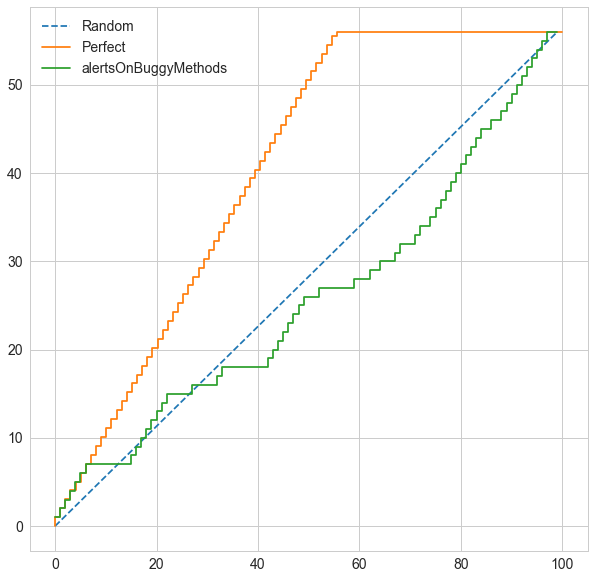
\includegraphics[scale=0.3]{./src/methodBug/methodbug_cumulative_graph_top100.png}
		\caption{Cumulative graph for the first 100 alerts}\label{}
	\end{subfigure}\\
	\begin{subfigure}{.5\textwidth}
		\centering
		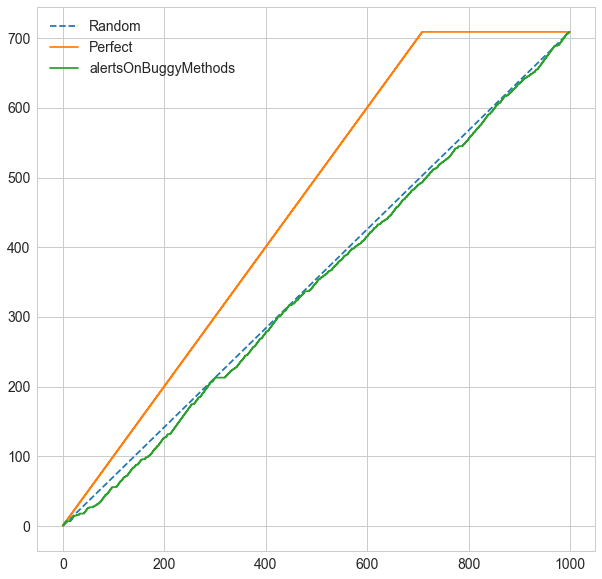
\includegraphics[scale=0.3]{./src/methodBug/methodbug_cumulative_graph_top1000.png}
		\caption{Cumulative graph for the first 1000 alerts}\label{}
	\end{subfigure}%
	\begin{subfigure}{.5\textwidth}
		\centering
		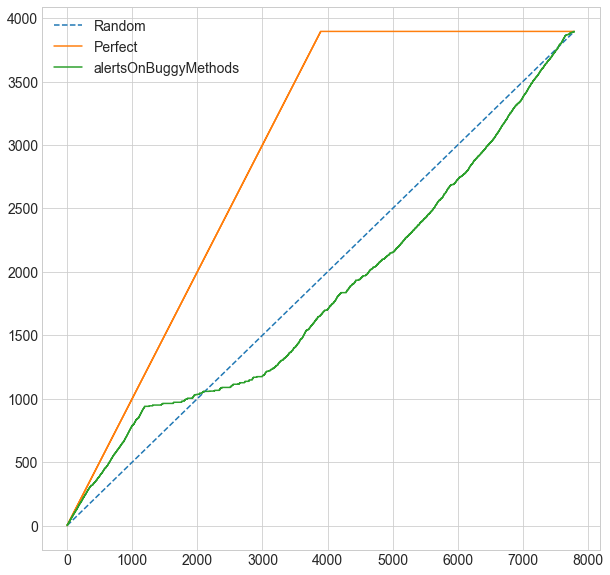
\includegraphics[scale=0.3]{./src/methodBug/methodbug_cumulative_graph_all.png}
		\caption{Cumulative graph for all alerts}\label{}
	\end{subfigure}  
\end{figure}

From the results we can conclude that ranking alerts based on the method being bug-prone does not provide good results. That does not mean that this method is meaningless. Its main purpose is to give extra attention to alerts belonging to buggy methods, which if acted upon may improve code quality and lower the probability of the method causing a bug in the future.

\subsection{Feedback Rank}

\textit{(*) These experiments were run on a small subset of the dataset. The Bayes Network was trained on 10000 samples and tested on 1000. The reason being the abnormally high runtime (factor 100 or more than other approaches).}

Different balancing algorithms were applied to the training set and \textit{Bayes Network} was used as a classifier. The following results show the score of the classifier:

\begin{table}[H]
	\centering
	\begin{tabular}{ccccccc}
		\hline
		& \textbf{Precision} & \textbf{Recall} & \textbf{Specificity} & \textbf{F1-Score} & \textbf{Geometric} & \textbf{IBA}  \\ \hline
		\textit{Random Over Sampler}  & 56\%               & 53\%            & 56\%                 & 52\%              & 51\%               & 26\%          \\
		\textit{Random Under Sampler} & 57\%               & 54\%            & 57\%                 & 52\%              & 52\%               & 27\%          \\
		\textit{None}                 & \textbf{58\%}      & \textbf{56\%}   & \textbf{57\%}        & \textbf{54\%}     & \textbf{53\%}      & \textbf{28\%}
	\end{tabular}
\end{table}


\begin{figure}[H]
	\begin{subfigure}{\textwidth}
		\centering
		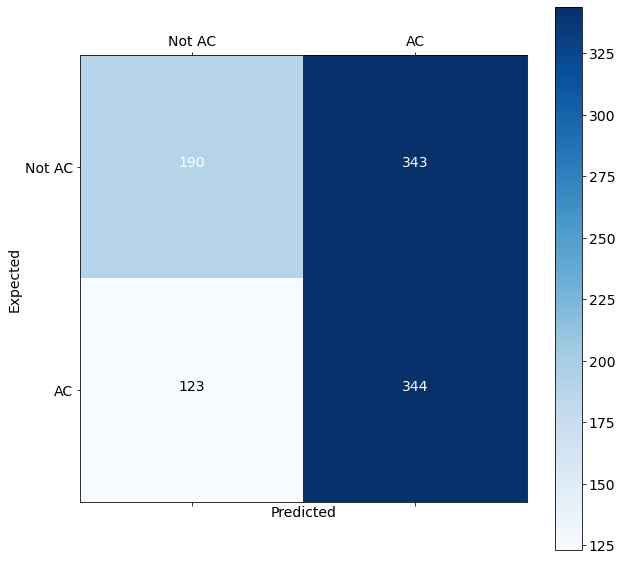
\includegraphics[scale=0.3]{./src/fbRank/fbrank_nob_cm.png}
		\caption{Confusion matrix of test set for unbalanced training set}\label{}
	\end{subfigure}\\
	\begin{subfigure}{.5\textwidth}
		\centering
		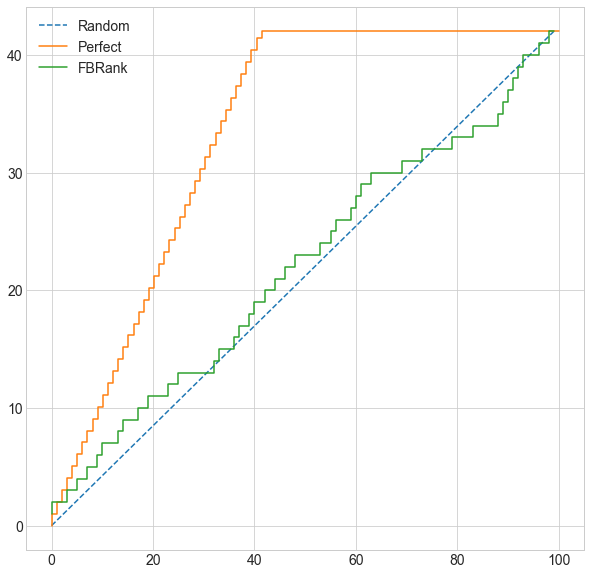
\includegraphics[scale=0.3]{./src/fbRank/fbrank_cumulative_graph_top100.png}
		\caption{Cumulative graph for the first 100 alerts}\label{}
	\end{subfigure}%
	\begin{subfigure}{.5\textwidth}
		\centering
		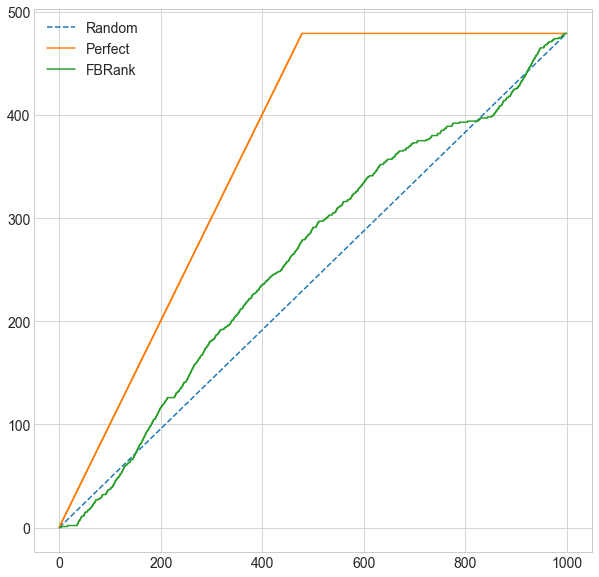
\includegraphics[scale=0.3]{./src/fbRank/fbrank_cumulative_graph_top1000.png}
		\caption{Cumulative graph for the first 1000 alerts}\label{}
	\end{subfigure}  
\end{figure}

\begin{table}[H]
	\centering
	\begin{tabular}{@{}lll@{}}
		\toprule
		& \textbf{S(R) metric} & \textbf{Average FP to TP} \\ \midrule
		\textit{Better than random (Top 100 alerts)}  & 1000 out of 1000       & 63 out of 1000           \\
		\textit{Better than random (Top 1000 alerts)} & 958 out of 1000      & 859 out of 1000          \\ \bottomrule
	\end{tabular}
\end{table}

From the metrics as well as the cumulative graph, we can see that Feedback Rank does not perform well on the reduced dataset it was tested on.


\subsection{Bug-Related Lines}

Since this method only calculates weights for alert types, it does not predict if a particular alert is actionable or not. As a consequence, only the ranking is evaluated.

The algorithm ranks alerts types based on two input weight parameters ($\alpha,\beta$). Based on experimental evaluation the following respective values were chosen: $\alpha=0.7, 
\beta=0.3$.

\begin{figure}[H]
	\begin{subfigure}{\textwidth}
		\centering
		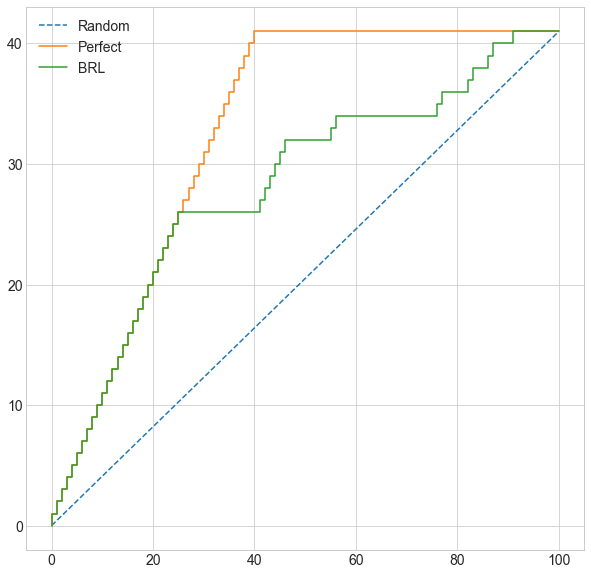
\includegraphics[scale=0.3]{./src/brls/brls_cumulative_graph_top100.png}
		\caption{Cumulative graph for the first 100 alerts}\label{}
	\end{subfigure}\\
	\begin{subfigure}{.5\textwidth}
		\centering
		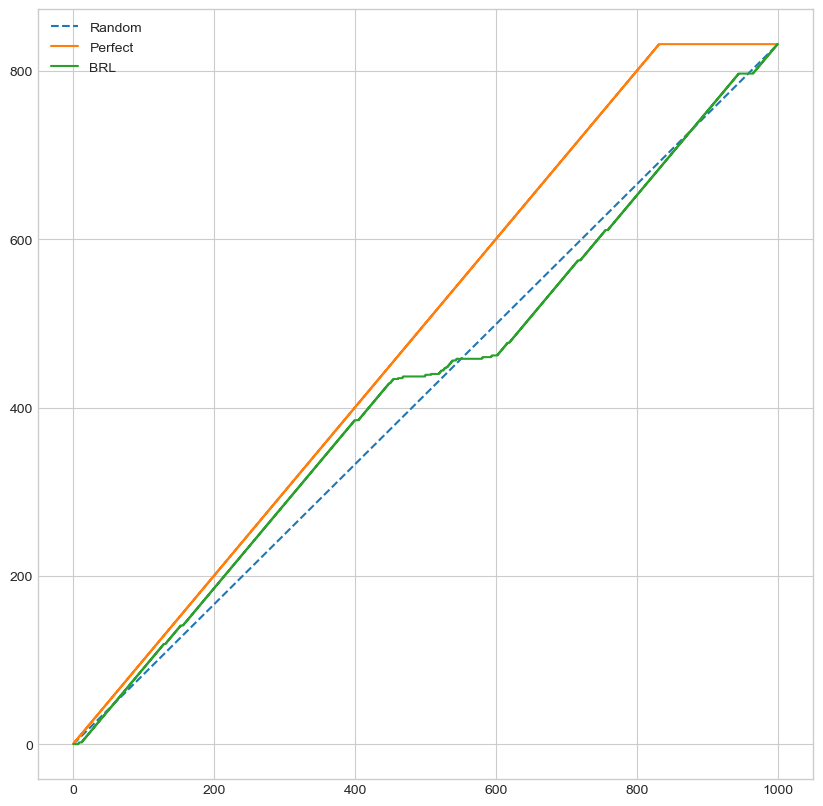
\includegraphics[scale=0.3]{./src/brls/brls_cumulative_graph_top1000.png}
		\caption{Cumulative graph for the first 1000 alerts}\label{}
	\end{subfigure}%
	\begin{subfigure}{.5\textwidth}
		\centering
		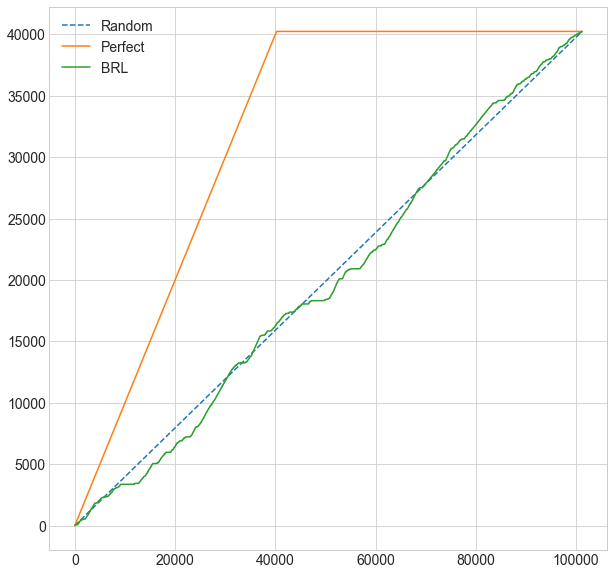
\includegraphics[scale=0.3]{./src/brls/brls_cumulative_graph_all.png}
		\caption{Cumulative graph for all alerts}\label{}
	\end{subfigure}  
\end{figure}

The algorithm performs well for the first 100 alerts, but then the performance decreases. 

\begin{table}[H]
	\centering
	\begin{tabular}{@{}lll@{}}
		\toprule
		& \textbf{S(R) metric} & \textbf{Average FP to TP} \\ \midrule
		\textit{Better than random (Top 100 alerts)}  & 1000 out of 1000       & 993 out of 1000           \\
		\textit{Better than random (Top 1000 alerts)} & 0 out of 1000      & 996 out of 1000          \\ \bottomrule
	\end{tabular}
\end{table}


\subsection{Combined technique}
\textbf{TO DOOOOOOO}